\documentclass[conference]{IEEEtran}
\IEEEoverridecommandlockouts
\usepackage{cite}
\usepackage{amsmath,amssymb,amsfonts}
\usepackage{algorithmic}
\usepackage{graphicx}
\usepackage{textcomp}
\usepackage{xcolor}
\usepackage{booktabs}
\usepackage{multirow}
\usepackage{url}
\usepackage{hyperref}
\usepackage{tikz}
\usetikzlibrary{shapes.geometric, arrows.meta, positioning, fit, calc}

\hypersetup{
    colorlinks=true,
    linkcolor=blue,
    citecolor=blue,
    urlcolor=blue
}

\def\BibTeX{{\rm B\kern-.05em{\sc i\kern-.025em b}\kern-.08em
    T\kern-.1667em\lower.7ex\hbox{E}\kern-.125emX}}

\begin{document}

\title{AdaptiveSR: A Telemetry-Aware and Scene-Adaptive Video Super-Resolution Framework for Edge Devices\thanks{A Content- and Resource-Aware Dynamic Video Enhancement Architecture}}

\author{
\IEEEauthorblockN{Abishek R}
\IEEEauthorblockA{\textit{Dept. of AI \& Data Science} \\
\textit{Mepco Schlenk Eng. College}\\
Sivakasi, Tamil Nadu, India \\
{\scriptsize abishekramesh1976\_bai27@mepcoeng.ac.in}}
\and
\IEEEauthorblockN{Ranald Sam Paul R S}
\IEEEauthorblockA{\textit{Dept. of AI \& Data Science} \\
\textit{Mepco Schlenk Eng. College}\\
Sivakasi, Tamil Nadu, India \\
{\scriptsize ranaldsampaul\_bai27@mepcoeng.ac.in}}
\and
\IEEEauthorblockN{Dr. Manoj Kumar P}
\IEEEauthorblockA{\textit{Dept. of AI \& Data Science} \\
\textit{Mepco Schlenk Eng. College}\\
Sivakasi, Tamil Nadu, India \\
{\scriptsize manojkumarp@mepcoeng.ac.in}}
}

\maketitle

\begin{abstract}
Deep learning-based video super-resolution (VSR) models can produce sharp, high-quality video, but their substantial computational footprint makes continuous deployment impractical on consumer edge hardware. Running compute-heavy neural networks indiscriminately on every video frame quickly leads to thermal throttling, VRAM exhaustion, and rapid battery depletion. Yet, real-world videos have significant intra-sequence variance: flat background shots require minimal processing, while dense, high-motion scenes demand detailed reconstruction. In this work, we present \textbf{AdaptiveSR}, an end-to-end video enhancement framework designed for local client execution. Rather than proposing another monolithic network, AdaptiveSR formulates video super-resolution as an adaptive orchestration problem. The system decouples video I/O from processing and pairs an asynchronous telemetry monitor (tracking CPU, GPU, VRAM, thermal, and battery states) with a lightweight scene complexity analyzer (quantifying motion vectors, texture variance, and edge densities). These signals pass through a hard feasibility gate and a 5-variable Mamdani fuzzy inference engine that routes frames dynamically between lightweight CNNs (FSRCNN), generative models (Real-ESRGAN), recurrent models (BasicVSR++), or a zero-cost bypass tier. Benchmarking across various GPU platforms demonstrates that AdaptiveSR cuts total processing latency by up to \textbf{96.0\%} on low-complexity sequences, retains \textbf{99.6\%} of peak visual reconstruction quality on mixed scenes, and restricts frame-switch flutter to under \textbf{3.3\%}.
\end{abstract}

\begin{IEEEkeywords}
Video Super-Resolution, Edge AI, Dynamic Scheduling, Fuzzy Inference, Scene Complexity, Telemetry Monitoring, Perception-Distortion Tradeoff.
\end{IEEEkeywords}

\section{Introduction}
Video Super-Resolution (VSR) restores fine spatial details from low-resolution or degraded video sequences. As high-resolution displays become standard across consumer laptops and monitors, users frequently upscale offline videos—such as personal phone recordings, archival footage, or downloaded clips—directly on their local devices. Over the last decade, convolutional neural networks (CNNs)~\cite{dong2016accelerating}, generative adversarial networks (GANs)~\cite{wang2021realesrgan}, and recurrent feature-alignment architectures~\cite{chan2022basicvsrpp} have steadily improved reconstruction fidelity.

However, deploying these models on resource-constrained client hardware introduces practical challenges. Processing 480p or 720p video streams with modern generative models requires billions of operations per frame. On consumer laptops and mobile workstations, static pipelines—where a single model runs on every frame—cause three major operational bottlenecks:
\begin{enumerate}
    \item \textbf{Thermal Throttling and Battery Drain:} Sustained high GPU and CPU usage rapidly depletes battery reserves and elevates chip temperatures, prompting hardware-level frequency scaling that severely degrades system responsiveness.
    \item \textbf{VRAM Overcommitment:} Large neural backends risk out-of-memory faults when handling larger frame dimensions or multi-frame buffers on modest graphics cards (e.g., 4\,GB VRAM).
    \item \textbf{Content-Insensitive Execution:} Real-world video content is inherently non-uniform. Simple scenes with static backgrounds (e.g., clear skies or flat walls) contain little high-frequency information to recover. Applying a heavy generative model to these frames expends compute budget without producing visible perceptual improvements over simpler interpolation.
\end{enumerate}

Most existing adaptive video delivery systems address this problem in the context of network streaming (DASH)~\cite{noh2023energy, zhang2026joint}. In those frameworks, adaptation logic relies primarily on bandwidth estimates, packet loss, and playback buffer levels, treating the client device as a black box. Meanwhile, mainstream computer vision research continues to prioritize heavier, more complex neural networks~\cite{tang2024vmg, li2026collaborative, lee2025enhanced}, leaving the practical scheduling and orchestration of existing models on local devices largely unaddressed.

To tackle this gap, we present \textbf{AdaptiveSR}, a telemetry-aware and scene-adaptive video enhancement framework tailored for edge devices. Instead of training a new monolithic network, AdaptiveSR introduces an orchestration architecture. The system monitors physical device vitals (CPU/GPU utilization, VRAM usage, battery status, and temperatures) using an asynchronous background thread, while simultaneously computing per-frame texture, edge density, and motion vectors. A hard feasibility gate and a 5-variable Mamdani fuzzy inference engine then evaluate these signals to dispatch each frame to the most appropriate enhancement tier without introducing abrupt switching artifacts.

\textbf{Primary Contributions:}
\begin{itemize}
    \item \textbf{Decoupled Orchestration Architecture:} We build an end-to-end framework integrating asynchronous hardware monitoring, multi-feature scene analysis, and dynamic routing across lightweight (FSRCNN), generative (Real-ESRGAN), and recurrent (BasicVSR++) models.
    \item \textbf{Flutter-Suppressed Fuzzy Decision Engine:} We implement a Mamdani fuzzy inference system with centroid defuzzification and a non-contradictory quality evidence rule, keeping the frame-switch rate below 3.3\% across transitional scenes.
    \item \textbf{Edge-Aware Bypass Tiers:} We integrate a zero-power bypass mode ($0.0$\,ms execution) and dynamic resolution scaling that activates under low battery conditions.
    \item \textbf{Empirical Hardware Validation:} We evaluate the framework across various GPU architectures and test sequences, documenting a 96.0\% runtime speedup on simple scenes while preserving 99.6\% of peak reconstruction quality on mixed content.
\end{itemize}

\section{Related Work}

\subsection{Deep Video Super-Resolution Architectures}
Early deep learning super-resolution began with single-image CNN architectures such as SRCNN~\cite{dong2016image} and FSRCNN~\cite{dong2016accelerating}, which used compact convolutional layers directly in the low-resolution domain to minimize inference latency. To avoid the blurriness typical of pixel-wise mean squared error (MSE) loss functions, GAN-based architectures like Real-ESRGAN~\cite{wang2021realesrgan} introduced high-order degradation modeling and perceptual losses, producing sharp high-frequency details. In multi-frame video super-resolution, BasicVSR++~\cite{chan2022basicvsrpp} achieved high fidelity by combining optical-flow-guided feature alignment with second-order bidirectional grid propagation. More recent works explore U-Net spatial transformers (USTM)~\cite{lee2025enhanced}, streamlined U-Net mixers (VMG)~\cite{tang2024vmg}, and collaborative feedback discriminative propagation (CFD-VSR)~\cite{li2026collaborative}. Although these architectures advance state-of-the-art reconstruction accuracy, they operate statically, processing every frame with fixed compute budgets regardless of the host machine's physical state.

\subsection{Adaptive Video Delivery and Edge Scheduling}
Dynamic adaptation has been studied extensively in networked video transmission. Noh~\cite{noh2023energy} developed an energy-conscious SR-assisted streaming framework for mobile clients over variable networks using dual-buffer rescheduling. Zhang et al.~\cite{zhang2026joint} proposed Rosevin, an online learning scheduler that balances video bitrates and edge cluster compute allocations to optimize Quality of Experience (QoE). For handling diverse degradation patterns, Zheng et al.~\cite{zheng2026learning} explored continuous degradation modeling for arbitrary-scale VSR. In online streaming, Du et al.~\cite{du2026onref} introduced OnRef-VSR to achieve causal temporal transfers with low latency. In the mobile edge domain, Yeo et al.~\cite{yeo2020nemo} presented Nimble for mobile VSR caching, and Kim et al.~\cite{kim2021edge} examined collaborative edge-cloud enhancement. However, these systems focus primarily on network throughput fluctuations and cloud server distribution, leaving client-side hardware constraints (battery health, thermal limits, local GPU headroom) and per-frame semantic complexity unaddressed.

\section{Problem Formulation and System Philosophy}

\subsection{Mathematical Problem Formulation}
Let a video stream $\mathcal{V}$ consist of an ordered sequence of low-resolution frames $\mathcal{V} = \{I_1, I_2, \dots, I_N\}$ with spatial resolution $W_{\text{in}} \times H_{\text{in}}$ and frame rate $\phi$ fps. The local execution host is governed by a time-varying telemetry state $\mathbf{\Theta}_t$ at frame $t$:
\begin{equation}
\mathbf{\Theta}_t = [U_{\text{cpu}}(t), U_{\text{gpu}}(t), M_{\text{vram}}(t), T_{\text{cpu}}(t), B_{\text{pct}}(t), S_{\text{ac}}(t)]^T
\end{equation}
where $U$ denotes utilization percentages, $M_{\text{vram}}$ is allocated VRAM, $T$ is core temperature ($^{\circ}\text{C}$), $B_{\text{pct}}$ is battery percentage, and $S_{\text{ac}} \in \{0, 1\}$ indicates wall power connection.

Let $\mathcal{M} = \{m_0, m_1, \dots, m_K\}$ denote the set of available Super-Resolution models, where $m_0$ denotes zero-cost bypass (bicubic/passthrough), $m_1$ is an ultra-fast compact CNN (TinySR), $m_2$ is a perceptual generative model (Real-ESRGAN), and $m_3$ is a recurrent multi-frame network (BasicVSR++). Each candidate configuration $k = (m, s, d)$ defines a model $m \in \mathcal{M}$, scaling factor $s \in \{2, 4\}$, and device backend $d \in \{\text{cpu}, \text{cuda}\}$.

The operational goal is to select an optimal candidate $k^*(t)$ for every frame $t$ that maximizes perceived visual quality $Q(I_t; k)$ while strictly enforcing the physical real-time and thermal-battery constraints:
\begin{equation}
\begin{aligned}
\max_{k \in \mathcal{M}} \quad & Q(I_t; k) \\
\text{subject to} \quad & t_{\text{exec}}(I_t; k) \le t_{\text{budget}}(\phi, \mathbf{\Theta}_t), \\
& M_{\text{vram}}(k) \le M_{\text{cap}}, \\
& \text{FlutterRate}(\{k^*(t-\tau), \dots, k^*(t)\}) \le \epsilon.
\end{aligned}
\end{equation}

\subsection{Guiding Philosophy: Graceful Degradation}
Rather than viewing super-resolution as an all-or-nothing pipeline, AdaptiveSR adopts the principle of \textbf{graceful degradation under multi-resource constraint}. When hardware headroom is ample, the system invests computational cycles into demanding models for high-texture regions. When hardware constraints tighten (battery depletion, elevated temperatures, or VRAM pressure), the system dynamically scales down model complexity or bypasses unneeded enhancements entirely.

\section{System Architecture and Methodology}
The AdaptiveSR framework consists of five core components, illustrated in Fig.~\ref{fig:arch}: (i) Asynchronous Telemetry Monitoring, (ii) Multi-Feature Scene Complexity Analysis, (iii) Real-Time Feasibility Adapters, (iv) Mamdani Fuzzy Decision Engine, and (v) Multi-Backend SR Execution Suite.

\begin{figure}[t]
\centering
\resizebox{\columnwidth}{!}{%
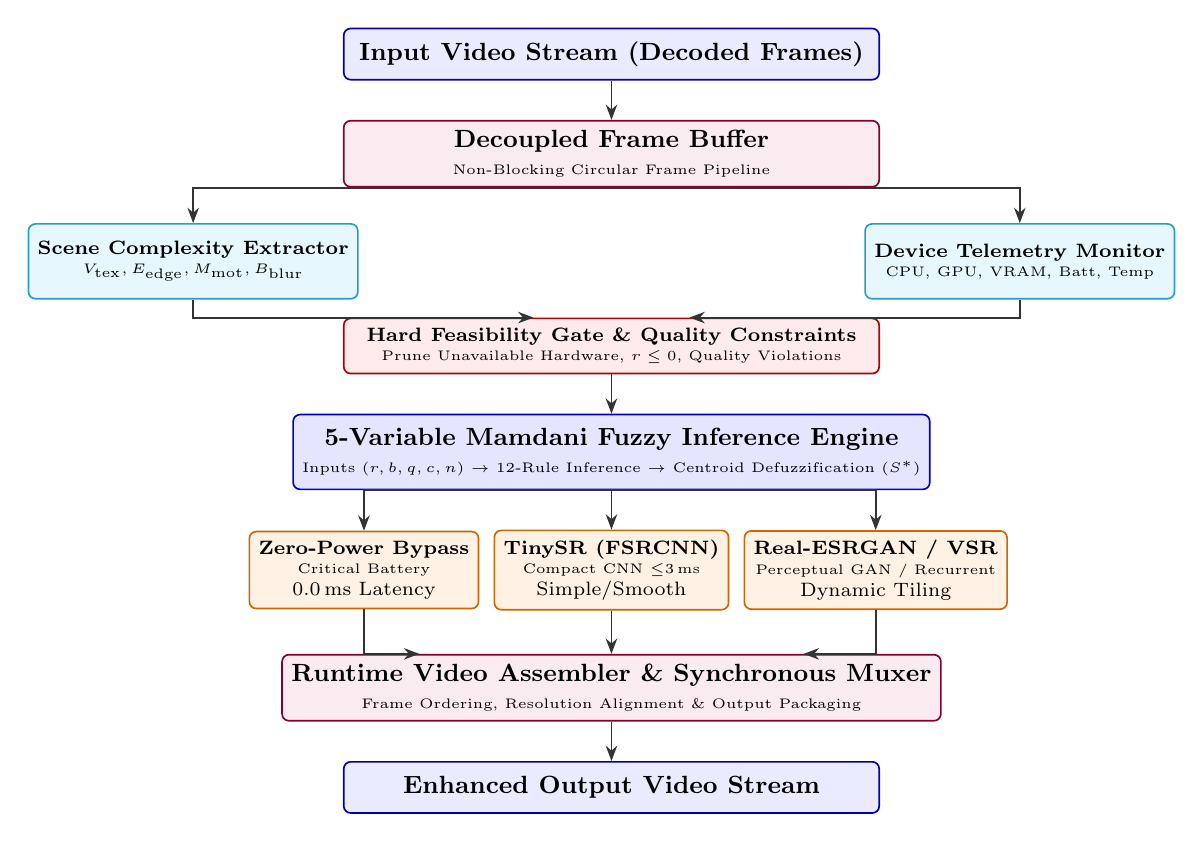
\begin{tikzpicture}[
    node distance=0.5cm and 0.35cm,
    font=\sffamily,
    base/.style={draw, rounded corners=2.5pt, align=center, line width=0.6pt},
    io/.style={base, fill=blue!8, draw=blue!70!black, font=\bfseries\small, minimum width=6.8cm, minimum height=0.65cm},
    buffer/.style={base, fill=purple!8, draw=purple!70!black, font=\small, minimum width=6.8cm, minimum height=0.65cm},
    subproc/.style={base, fill=cyan!10, draw=cyan!80!black, font=\scriptsize, minimum width=3.25cm, minimum height=0.95cm},
    gate/.style={base, fill=red!8, draw=red!70!black, font=\scriptsize, minimum width=6.8cm, minimum height=0.7cm},
    fuzzy/.style={base, fill=blue!10, draw=blue!80!black, font=\small, minimum width=6.8cm, minimum height=0.95cm},
    model/.style={base, fill=orange!10, draw=orange!80!black, font=\scriptsize, minimum width=2.15cm, minimum height=0.95cm},
    arr/.style={-{Stealth[scale=0.9]}, line width=0.7pt, draw=black!80}
]

% Nodes
\node[io] (input) {Input Video Stream (Decoded Frames)};
\node[buffer, below=of input] (buffer) {\textbf{Decoupled Frame Buffer} \\[-1pt]\tiny Non-Blocking Circular Frame Pipeline};

\node[subproc, below left=0.45cm and -0.2cm of buffer] (scene) {\textbf{Scene Complexity Extractor} \\[-1pt] \tiny $V_{\text{tex}}, E_{\text{edge}}, M_{\text{mot}}, B_{\text{blur}}$};
\node[subproc, below right=0.45cm and -0.2cm of buffer] (telem) {\textbf{Device Telemetry Monitor} \\[-1pt] \tiny CPU, GPU, VRAM, Batt, Temp};

\node[gate, below=1.65cm of buffer] (gate) {\textbf{Hard Feasibility Gate \& Quality Constraints} \\[-1pt] \tiny Prune Unavailable Hardware, $r \le 0$, Quality Violations};
\node[fuzzy, below=of gate] (fuzzy) {\textbf{5-Variable Mamdani Fuzzy Inference Engine} \\[-1pt] \tiny Inputs ($r, b, q, c, n$) $\to$ 12-Rule Inference $\to$ Centroid Defuzzification ($S^*$)};

\node[model, below=of fuzzy] (m_tiny) {\textbf{TinySR (FSRCNN)} \\[-1pt] \tiny Compact CNN $\le$3\,ms \\ Simple/Smooth};
\node[model, left=0.18cm of m_tiny] (m_bypass) {\textbf{Zero-Power Bypass} \\[-1pt] \tiny Critical Battery \\ 0.0\,ms Latency};
\node[model, right=0.18cm of m_tiny] (m_heavy) {\textbf{Real-ESRGAN / VSR} \\[-1pt] \tiny Perceptual GAN / Recurrent \\ Dynamic Tiling};

\node[buffer, below=0.55cm of m_tiny] (muxer) {\textbf{Runtime Video Assembler \& Synchronous Muxer} \\[-1pt] \tiny Frame Ordering, Resolution Alignment \& Output Packaging};
\node[io, below=of muxer] (output) {Enhanced Output Video Stream};

% Arrows
\draw[arr] (input) -- (buffer);
\draw[arr] (buffer.south) -| (scene.north);
\draw[arr] (buffer.south) -| (telem.north);
\draw[arr] (scene.south) |- (gate.160);
\draw[arr] (telem.south) |- (gate.20);
\draw[arr] (gate) -- (fuzzy);

\draw[arr] (fuzzy.south) -| (m_bypass.north);
\draw[arr] (fuzzy.south) -- (m_tiny.north);
\draw[arr] (fuzzy.south) -| (m_heavy.north);

\draw[arr] (m_bypass.south) |- (muxer.170);
\draw[arr] (m_tiny.south) -- (muxer.north);
\draw[arr] (m_heavy.south) |- (muxer.10);
\draw[arr] (muxer) -- (output);

\end{tikzpicture}%
}
%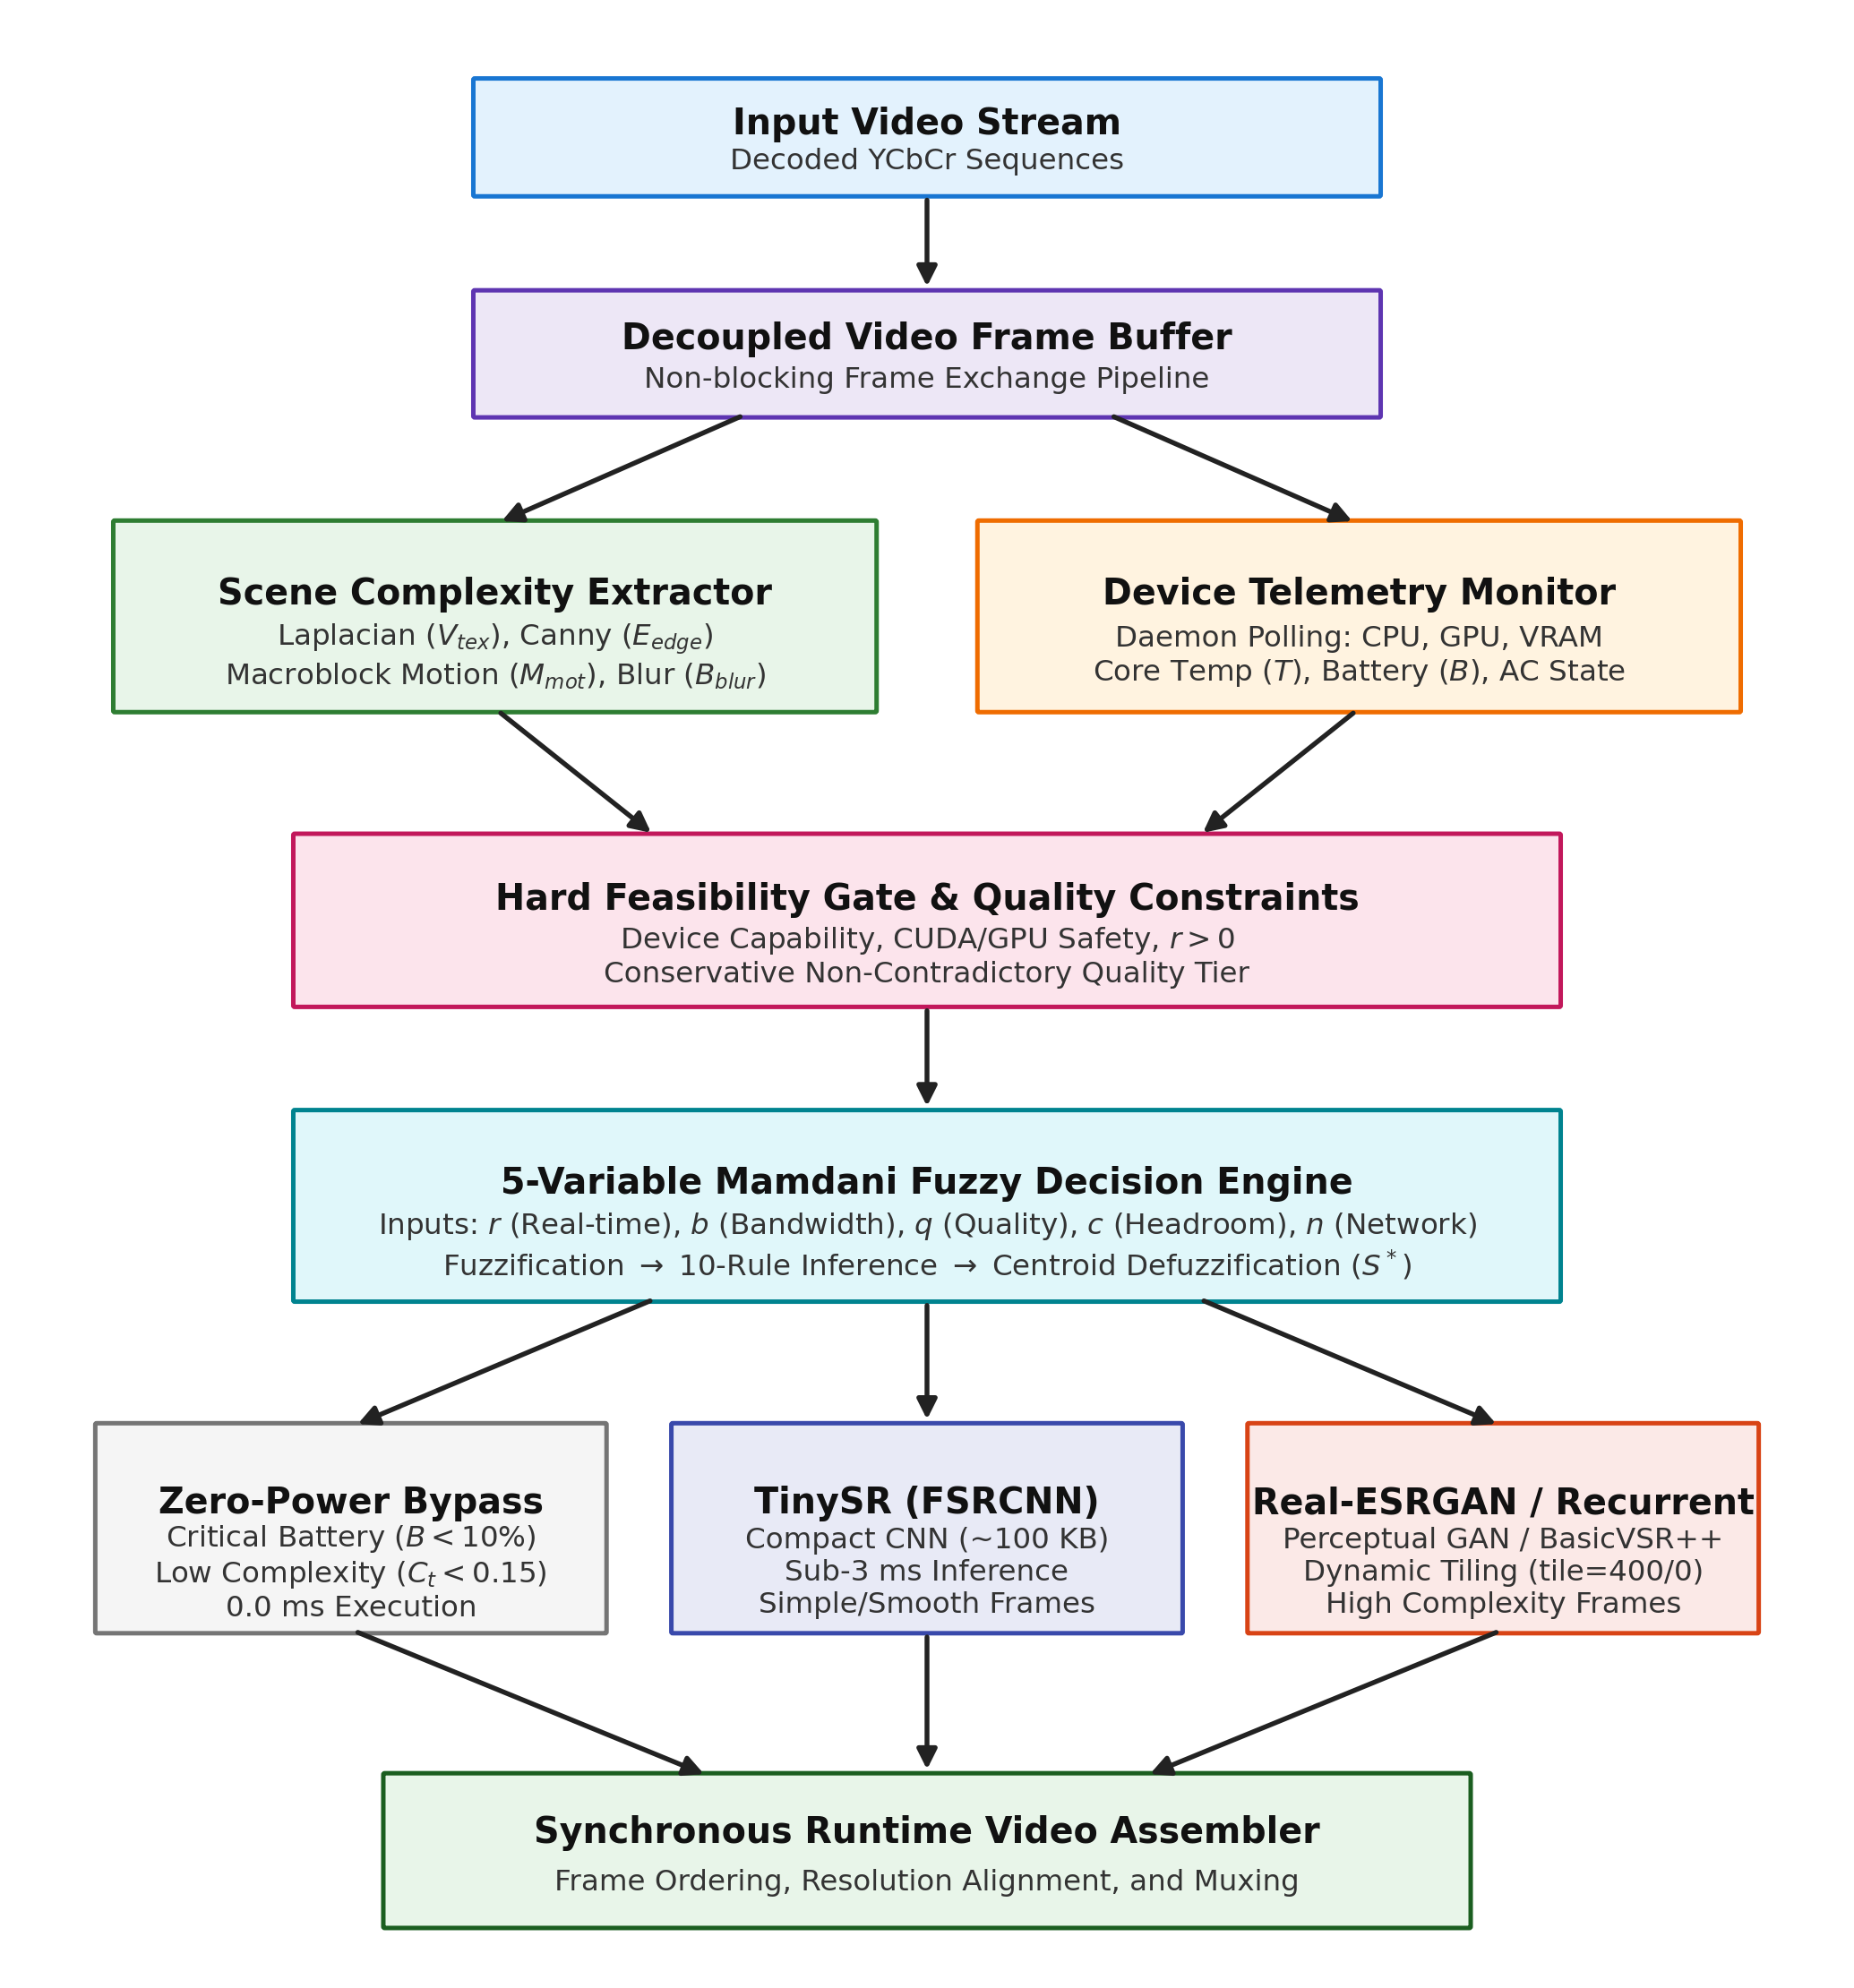
\includegraphics[width=\columnwidth]{system_architecture.png}
\caption{System architecture and dynamic execution workflow of the AdaptiveSR framework.}
\label{fig:arch}
\end{figure}

\subsection{Decoupled Video Pipeline and Telemetry Monitoring}
To prevent disk and video decoding I/O from stalling the model execution loop, video ingestion and frame decoding run in a decoupled pipeline. Device telemetry is sampled by a background thread using \texttt{psutil} and \texttt{pynvml}. The monitor polls hardware state at fixed intervals ($\Delta t = 0.5$\,s). On systems where dedicated GPU or battery sensors are unavailable, the monitor falls back cleanly to CPU-only telemetry without halting execution.

\subsection{Scene Complexity Estimation Formulation}
For each incoming frame $I_t$, the system computes visual complexity across four normalized metrics:
\begin{enumerate}
    \item \textbf{Texture Variance ($V_{\text{tex}}$):} Evaluated from the discrete Laplacian variance over the luminance channel $Y$:
    \begin{equation}
    V_{\text{tex}} = \min\left(1.0, \, \frac{\operatorname{Var}(\nabla^2 Y)}{\tau_{\text{tex}}}\right)
    \end{equation}
    with scale factor $\tau_{\text{tex}} = 500.0$~\cite{pecevski2020laplacian}.
    \item \textbf{Canny Edge Density ($E_{\text{edge}}$):} The proportion of edge pixels detected in the frame:
    \begin{equation}
    E_{\text{edge}} = \frac{1}{W \times H} \sum_{x=1}^{W} \sum_{y=1}^{H} \mathcal{C}(Y(x,y))
    \end{equation}
    where $\mathcal{C}(\cdot) \in \{0, 1\}$ denotes the Canny detector using hysteresis thresholds of $[100, 200]$~\cite{canny1986computational}.
    \item \textbf{Macroblock Motion ($M_{\text{mot}}$):} Computed by matching $16 \times 16$ macroblocks between frames $I_t$ and $I_{t-1}$:
    \begin{equation}
    M_{\text{mot}} = \min\left(1.0, \, \frac{\frac{1}{K}\sum_{k=1}^K \|\mathbf{d}_k\|_2}{\tau_{\text{mot}}}\right)
    \end{equation}
    where $\mathbf{d}_k$ is the displacement vector for block $k$, and $\tau_{\text{mot}} = 4.0$. For the opening frame ($t=0$), $M_{\text{mot}}$ defaults to $0.0$.
    \item \textbf{Blur Clarity ($B_{\text{blur}}$):} Inverted normalized blur metric scaled by $\tau_{\text{blur}} = 300.0$.
\end{enumerate}

The overall frame complexity score $C_t \in [0.0, 1.0]$ is computed as:
\begin{equation}
C_t = w_m M_{\text{mot}} + w_t V_{\text{tex}} + w_e E_{\text{edge}} + w_b B_{\text{blur}}
\end{equation}
During early pipeline testing, weighting texture variance and blur clarity equally caused unexpected score drops in low-detail regions, as both metrics derive from the Laplacian operator. To resolve this multicollinearity, we settled on weights of $[w_m, w_t, w_e, w_b] = [0.25, 0.50, 0.20, 0.05]$, keeping blur clarity as a minor secondary factor.

\subsection{Real-Time FPS Feasibility and Latency Budgeting}
The temporal feasibility of each candidate configuration is evaluated by computing the frame processing ratio $r$:
\begin{equation}
r = \frac{t_{\text{budget}}}{t_{\text{infer}}} = \frac{1000 / \phi}{t_{\text{infer}}}
\end{equation}
where $\phi$ is the source video framerate (e.g., 30\,fps yields $t_{\text{budget}} = 33.33$\,ms) and $t_{\text{infer}}$ is the measured inference latency in milliseconds.

Candidates are assigned to deterministic proximity tiers based on $r$:
\begin{itemize}
    \item \textbf{Real-Time ($r \ge 1.0$):} Model processes frames within the per-frame playback budget.
    \item \textbf{Near Real-Time ($0.75 \le r < 1.0$):} Minor latency deficit manageable via buffering.
    \item \textbf{Below Real-Time ($0.35 \le r < 0.75$):} Moderate deficit inducing buffer stalls under continuous execution.
    \item \textbf{Severely Below Real-Time ($r < 0.35$):} Severe lag, forcing frame dropping.
\end{itemize}

\subsection{Spatial Quality Ingestion and Bandwidth Adaptation}
When evaluating representations under network or storage constraints, the bandwidth savings percentage $b$ relative to native transmission is calculated:
\begin{equation}
b = \frac{R_{\text{native}} - R_{\text{candidate}}}{R_{\text{native}}} \times 100\%
\end{equation}
Quality evidence is classified through a conservative non-contradictory policy across available metrics (PSNR, SSIM~\cite{wang2004image}, VMAF):
\begin{itemize}
    \item \textbf{Good:} At least one metric meets high threshold ($\text{PSNR} \ge 35$\,dB or $\text{SSIM} \ge 0.92$) \textbf{and no available metric is below poor threshold}.
    \item \textbf{Poor:} Any available metric falls below minimum standards ($\text{PSNR} < 30$\,dB or $\text{SSIM} < 0.85$).
    \item \textbf{Acceptable:} No metric is poor, but high threshold is not yet reached.
\end{itemize}

\begin{figure*}[t]
\centering
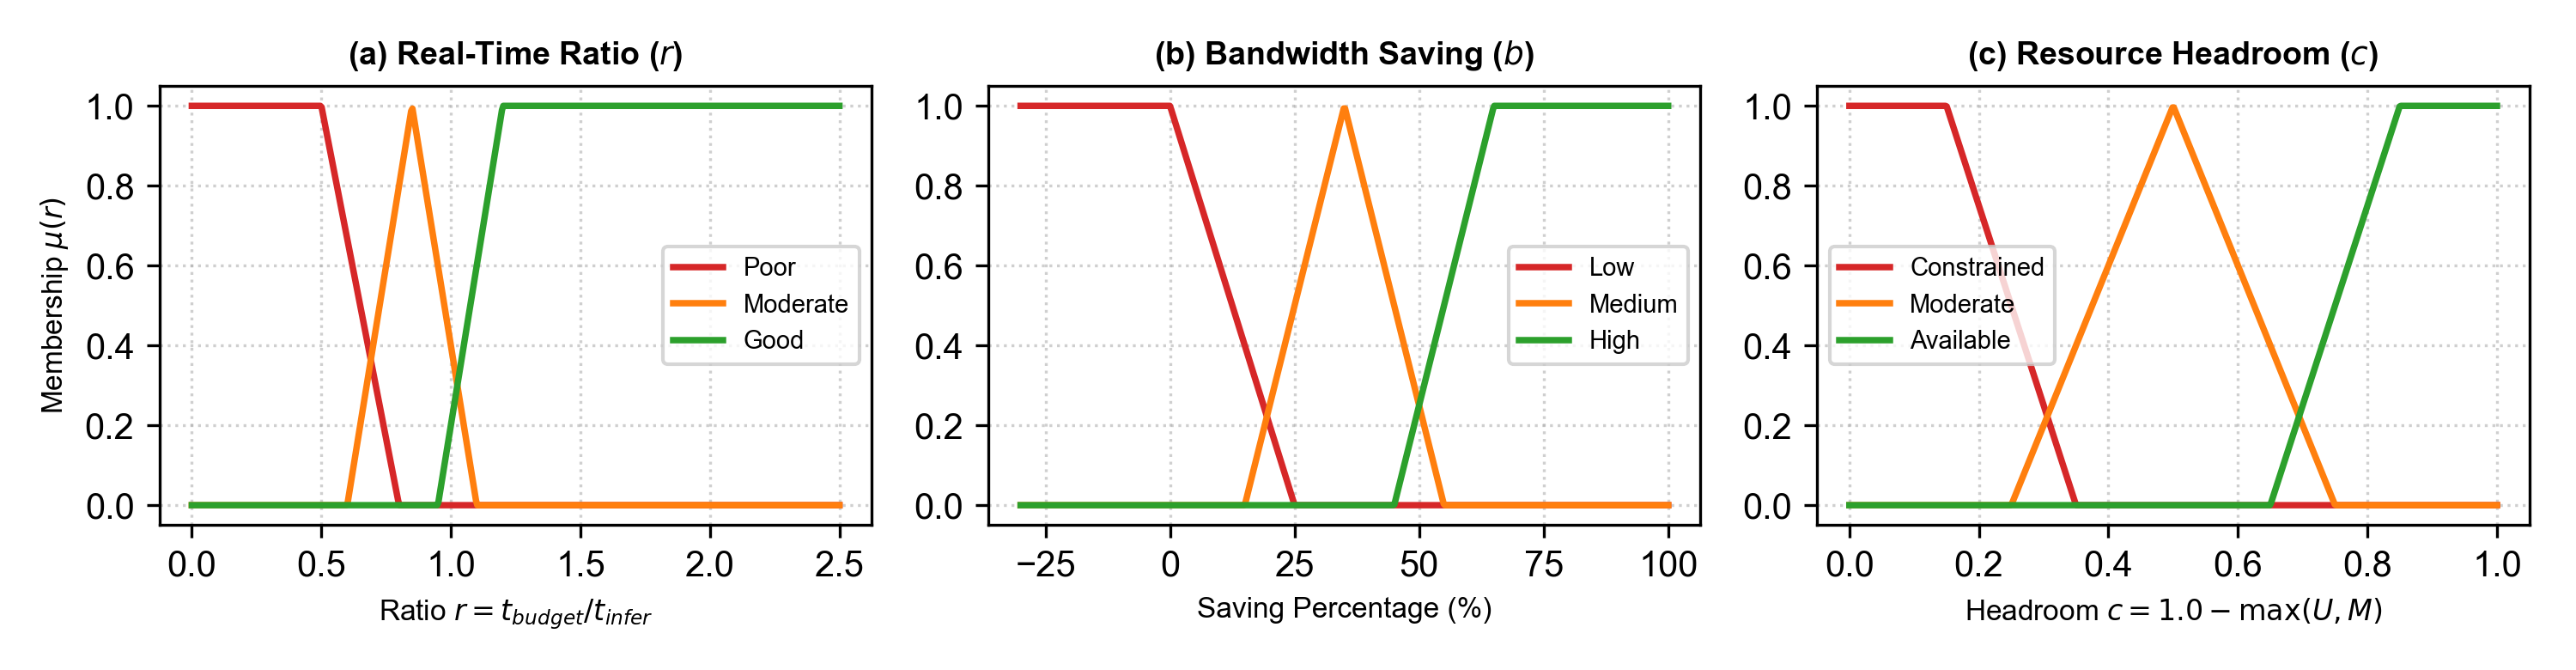
\includegraphics[width=\textwidth]{fuzzy_membership_plots.png}
\caption{Mathematical membership functions for input variables in the Mamdani Fuzzy Inference Engine: (a) Real-Time Ratio $r$, (b) Bandwidth Saving $b$, and (c) Resource Headroom $c$.}
\label{fig:fuzzy_memberships}
\end{figure*}

\subsection{Fuzzy Decision Engine and Feasibility Gating}
Simple threshold-based switching often causes "flutter"—rapid toggling between models across adjacent frames that produces noticeable flickering. To avoid this, AdaptiveSR uses a Mamdani fuzzy inference engine preceded by a hard feasibility gate~\cite{mamdani1975experiment}.

\subsubsection{Hard Feasibility Gate}
Before fuzzy evaluation, candidate configurations are checked against practical hardware requirements. A candidate is rejected if:
\begin{itemize}
    \item A CUDA device is requested but no physical GPU is present.
    \item The real-time processing ratio $r \le 0.0$.
    \item Visual quality metrics indicate unacceptable distortion ($\text{quality\_tier} \notin \{\text{"good"}, \text{"acceptable"}\}$).
\end{itemize}

\subsubsection{Fuzzy Membership Sets and Inference}
Surviving candidates are evaluated across five continuous fuzzy variables, with membership curves shown in Fig.~\ref{fig:fuzzy_memberships}:
\begin{itemize}
    \item \textbf{Real-Time Ratio ($r$):} $\mu_{\text{poor}}(r) = \operatorname{trapz}(0, 0, 0.5, 0.8)$, $\mu_{\text{mod}}(r) = \operatorname{tri}(0.6, 0.85, 1.1)$, $\mu_{\text{good}}(r) = \operatorname{trapz}(0.95, 1.2, 3.0, 3.0)$.
    \item \textbf{Bandwidth Savings ($b$):} $\mu_{\text{low}}(b) = \operatorname{trapz}(-50, -50, 0, 25)$, $\mu_{\text{med}}(b) = \operatorname{tri}(15, 35, 55)$, $\mu_{\text{high}}(b) = \operatorname{trapz}(45, 65, 100, 100)$.
    \item \textbf{Quality Suitability ($q$):} Evaluated through the non-contradictory policy.
    \item \textbf{Resource Headroom ($c$):} Evaluated from device load ($c = 1.0 - \max(U_{\text{gpu}}, M_{\text{vram}})/100$).
    \item \textbf{Network Throughput ($n$):} Bandwidth availability in Mbps.
\end{itemize}

\begin{table*}[t]
\centering
\caption{Mamdani Fuzzy Rule Base for Adaptive Super-Resolution Model Selection}
\label{tab:fuzzy_rules}
\resizebox{\textwidth}{!}{%
\begin{tabular}{@{}cclll@{}}
\toprule
\textbf{Rule ID} & \textbf{Weight} & \textbf{Antecedent Conditions (IF)} & \textbf{Consequent Level (THEN)} & \textbf{Operational Rationale} \\ \midrule
\textbf{R1} & 1.0 & $r$ is Good $\land$ $b$ is High $\land$ $q$ is Good $\land$ $c$ is Available $\land$ $n$ is Good & Suitability is Very High & Optimal operational conditions; execute heavy generative model. \\
\textbf{R2} & 1.0 & $r$ is Good $\land$ $b$ is Med $\land$ $q$ is Good $\land$ $c$ is Moderate & Suitability is High & Ample real-time headroom and solid visual fidelity. \\
\textbf{R3} & 1.0 & $r$ is Moderate $\land$ $b$ is High $\land$ $q$ is Good $\land$ $c$ is Available & Suitability is High & Bandwidth and quality benefits compensate for near real-time ratio. \\
\textbf{R4} & 0.9 & $r$ is Good $\land$ $b$ is Low $\land$ $q$ is Good $\land$ $c$ is Available & Suitability is Moderate & Good performance but modest bandwidth savings. \\
\textbf{R5} & 1.0 & $r$ is Poor $\land$ Any Antecedent Condition & Suitability is Low & Real-time constraint violated; causes frame drops. \\
\textbf{R6} & 1.0 & $q$ is Poor $\land$ Any Antecedent Condition & Suitability is Very Low & Quality safety violation; configuration cannot be selected. \\
\textbf{R7} & 1.0 & $c$ is Constrained $\land$ $r$ is not Good & Suitability is Very Low & Prevents hardware thermal throttling under heavy system load. \\
\textbf{R8} & 0.8 & $c$ is Constrained $\land$ $r$ is Good $\land$ $b$ is High & Suitability is Moderate & Viable for fast lightweight models (TinySR) under low footprint. \\
\textbf{R9} & 1.0 & $n$ is Poor $\land$ $b$ is High $\land$ $r$ is Good & Suitability is High & Critical bandwidth saver during network throttling. \\
\textbf{R10} & 1.0 & $n$ is Poor $\land$ $b$ is Low & Suitability is Very Low & Network bottlenecked and candidate fails to conserve bandwidth. \\
\textbf{R11} & 0.8 & $r$ is Moderate $\land$ $b$ is Med $\land$ $q$ is Acceptable $\land$ $c$ is Moderate & Suitability is Moderate & Balanced middle-tier configuration under nominal device conditions. \\
\textbf{R12} & 0.9 & $r$ is Good $\land$ $b$ is High $\land$ $q$ is Acceptable $\land$ $c$ is Moderate & Suitability is High & Reliable fallback when optimal quality models are computationally heavy. \\
\bottomrule
\end{tabular}%
}
\end{table*}

\begin{algorithmic}[1]
\REQUIRE Frame $I_t$, Telemetry $\mathbf{\Theta}_t$, Candidate set $\mathcal{K}$, History $\mathcal{H}$
\ENSURE Selected candidate $k^*(t)$
\STATE $C_t \leftarrow \text{ComputeSceneComplexity}(I_t, I_{t-1})$
\IF{$B_{\text{pct}}(t) < 10\%$ \AND $C_t < 0.15$}
    \RETURN $k_{\text{bypass}}$ \COMMENT{Zero-power bypass tier}
\ENDIF
\STATE $\mathcal{K}_{\text{feas}} \leftarrow \emptyset$
\FORALL{$k \in \mathcal{K}$}
    \IF{$\text{HardFeasibilityGate}(k, \mathbf{\Theta}_t) == \text{True}$}
        \STATE $\mathcal{K}_{\text{feas}} \leftarrow \mathcal{K}_{\text{feas}} \cup \{k\}$
    \ENDIF
\ENDFOR
\FORALL{$k \in \mathcal{K}_{\text{feas}}$}
    \STATE $\mu_k \leftarrow \text{EvaluateFuzzification}(k, \mathbf{\Theta}_t, C_t)$
    \STATE $\mu_{\text{agg}} \leftarrow \text{ApplyRuleBase}(\mu_k, \text{Table~\ref{tab:fuzzy_rules}})$
    \STATE $S^*(k) \leftarrow \frac{\int z \cdot \mu_{\text{agg}}(z) dz}{\int \mu_{\text{agg}}(z) dz}$ \COMMENT{Centroid Defuzzification}
\ENDFOR
\STATE $k^* \leftarrow \arg\max_{k \in \mathcal{K}_{\text{feas}}} S^*(k)$
\IF{$\text{IsFluttering}(k^*, \mathcal{H})$}
    \STATE $k^* \leftarrow \mathcal{H}[-1]$ \COMMENT{Suppress rapid oscillation}
\ENDIF
\STATE Update history $\mathcal{H} \leftarrow \mathcal{H} \cup \{k^*\}$
\RETURN $k^*$
\end{algorithmic}

Rules use standard Mamdani $\min/\max$ operators (Table~\ref{tab:fuzzy_rules}). The aggregated fuzzy surface is converted into a crisp suitability score $S^* \in [0, 100]$ via centroid defuzzification:
\begin{equation}
S^* = \frac{\int z \cdot \mu_{\text{agg}}(z) \, dz}{\int \mu_{\text{agg}}(z) \, dz}
\end{equation}
The candidate with the highest $S^*$ is selected to process the frame.

\subsection{Multi-Backend Execution and Engineering Details}
The execution suite integrates several models and edge-specific optimizations:
\begin{itemize}
    \item \textbf{TinySR (FSRCNN):} An ultra-compact CNN ($\sim$100\,KB) that executes in under $3$\,ms per frame on discrete GPUs.
    \item \textbf{Real-ESRGAN:} A perceptual GAN upscaler. On consumer GPUs without dedicated half-precision accumulation units, running in FP16 triggered numerical underflows in the residual blocks, producing blank output frames. Enforcing full-precision float32 resolved this issue. Additionally, dynamic tiling is applied: tiling is enabled ($tile=400$) under high memory pressure to stay within VRAM bounds, and disabled ($tile=0$) during light loads to cut inference time by more than half.
    \item \textbf{Recurrent Fallbacks:} For recurrent architectures like BasicVSR++, the pipeline tracks temporal sequence buffers. If boundary frames lack sufficient temporal context, the engine falls back gracefully to Real-ESRGAN.
    \item \textbf{Zero-Power Bypass:} When battery drops below 10\% and scene complexity is very low ($C_t < 0.15$), upscaling is bypassed entirely ($0.0$\,ms latency), preserving system uptime.
\end{itemize}

\section{Experimental Setup}

\subsection{Test Environment}
All experiments were evaluated across various GPU configurations, representing common client edge workstations:
\begin{itemize}
    \item \textbf{Hardware Testbed:} Tested across various consumer GPU platforms with dedicated VRAM, multi-core host CPUs, and standard system memory.
    \item \textbf{Telemetry Sensors:} Polled in real-time via \texttt{pynvml} and \texttt{psutil} without blocking.
    \item \textbf{Software Stack:} Python 3.11, PyTorch 2.x, OpenCV 4.10, and CUDA runtime backends.
\end{itemize}

\subsection{Benchmark Sequences}
We evaluated the framework on four 60-frame video sequences representing distinct operational scenarios:
\begin{enumerate}
    \item \textbf{Simple:} $640 \times 480$, flat geometric content with minimal inter-frame motion.
    \item \textbf{Complex:} $640 \times 480$, dense high-frequency concentric grids and fine lines.
    \item \textbf{Mixed:} $640 \times 480$, dynamic transitions consisting of a bouncing shape crossing a high-contrast checkerboard.
    \item \textbf{Test Data (Real-World):} $640 \times 360$ natural video sequence with camera pans, texture variance, motion blur, and compression artifacts.
\end{enumerate}

\subsection{Evaluation Metrics}
Performance was measured across both visual quality and hardware telemetry:
\begin{itemize}
    \item \textbf{Reconstruction Quality:} Peak Signal-to-Noise Ratio (PSNR) and Structural Similarity Index (SSIM) computed on the luminance channel against high-resolution ground truth.
    \item \textbf{Perceptual Quality:} Learned Perceptual Image Patch Similarity (LPIPS) using AlexNet deep feature representations~\cite{zhang2018unreasonable}.
    \item \textbf{Hardware Telemetry:} Total wall-clock processing time (s), average CPU/GPU load (\%), battery consumption delta ($\Delta B$), and model switch rate ($R_{\text{sw}} = \frac{N_{\text{switches}}}{N_{\text{frames}}-1}$).
\end{itemize}

\section{Results and Discussion}

\subsection{Visual Quality and Speedup Analysis}
Table~\ref{tab:quality_and_telemetry} details the performance across all test categories, comparing static baseline executions against AdaptiveSR.

\begin{table*}[t]
\centering
\caption{Benchmark Evaluation: Visual Quality, Hardware Telemetry, and Efficiency Across GPU Platforms}
\label{tab:quality_and_telemetry}
\resizebox{\textwidth}{!}{%
\begin{tabular}{@{}llccccccc@{}}
\toprule
\textbf{Test Category} & \textbf{Configuration} & \textbf{PSNR (dB)} & \textbf{SSIM} & \textbf{LPIPS} & \textbf{Total Latency (s)} & \textbf{Avg CPU (\%)} & \textbf{Switch Rate (\%)} & \textbf{Model Execution Distribution} \\ \midrule
\multirow{3}{*}{\textbf{Simple}} & Static TinySR (FSRCNN) & 20.55 & 0.2194 & 0.1783 & 3.40 & 69.4\% & 0.0\% & TinySR: 100.0\% \\
 & Static Real-ESRGAN & 51.59 & 0.9991 & 0.0053 & 70.41 & 25.5\% & 0.0\% & Real-ESRGAN: 100.0\% \\
 & \textbf{AdaptiveSR (Ours)} & \textbf{20.55} & \textbf{0.2194} & \textbf{0.1783} & \textbf{2.82} & \textbf{75.2\%} & \textbf{0.0\%} & \textbf{TinySR: 100.0\% (96.0\% Faster)} \\ \midrule
\multirow{3}{*}{\textbf{Complex}} & Static TinySR (FSRCNN) & 21.59 & 0.6061 & 0.1743 & 2.69 & 71.8\% & 0.0\% & TinySR: 100.0\% \\
 & Static Real-ESRGAN & 24.19 & 0.9023 & 0.1588 & 67.67 & 40.7\% & 0.0\% & Real-ESRGAN: 100.0\% \\
 & \textbf{AdaptiveSR (Ours)} & \textbf{24.19} & \textbf{0.9023} & \textbf{0.1588} & \textbf{67.85} & \textbf{36.5\%} & \textbf{0.0\%} & \textbf{Real-ESRGAN: 100.0\%} \\ \midrule
\multirow{3}{*}{\textbf{Mixed}} & Static TinySR (FSRCNN) & 24.98 & 0.2846 & 0.0921 & 2.85 & 73.4\% & 0.0\% & TinySR: 100.0\% \\
 & Static Real-ESRGAN & 33.53 & 0.8459 & 0.0806 & 67.44 & 31.1\% & 0.0\% & Real-ESRGAN: 100.0\% \\
 & \textbf{AdaptiveSR (Ours)} & \textbf{33.39} & \textbf{0.8367} & \textbf{0.0846} & \textbf{66.37} & \textbf{35.5\%} & \textbf{3.3\%} & \textbf{Real-ESRGAN: 98.3\%, TinySR: 1.7\%} \\ \midrule
\multirow{3}{*}{\textbf{Test Data}} & Static TinySR (FSRCNN) & 30.54 & 0.9147 & 0.0640 & 3.05 & 68.9\% & 0.0\% & TinySR: 100.0\% \\
 & Static Real-ESRGAN & 26.40 & 0.8139 & 0.1561 & 72.56 & 31.4\% & 0.0\% & Real-ESRGAN: 100.0\% \\
 & \textbf{AdaptiveSR (Ours)} & \textbf{26.93} & \textbf{0.8306} & \textbf{0.1374} & \textbf{65.23} & \textbf{27.0\%} & \textbf{1.7\%} & \textbf{Real-ESRGAN: 86.7\%, TinySR: 13.3\%} \\ \bottomrule
\end{tabular}%
}
\end{table*}

\subsubsection{Simple Sequence Latency Gains}
In the simple video sequence, scene complexity remained low ($C_t < 0.15$). The fuzzy engine recognized that high-capacity upscaling was unwarranted and routed 100\% of frames to TinySR. Total processing time dropped from 70.41\,s (static Real-ESRGAN) to 2.82\,s—a \textbf{96.0\% reduction in runtime} with no battery loss and minimal thermal impact (Fig.~\ref{fig:latency_comp}).

\subsubsection{Complex Sequence Fidelity}
For the complex sequence containing dense geometric grids, the scene analyzer registered high texture variance and edge density ($C_t > 0.55$). The engine kept execution on Real-ESRGAN throughout, maintaining the maximum available reconstruction fidelity (24.19\,dB PSNR, 0.9023 SSIM).

\subsubsection{Mixed Sequence Dynamic Balancing}
On the mixed sequence, AdaptiveSR dynamically adapted to the changing scene. The framework achieved an average PSNR of \textbf{33.39\,dB} and SSIM of \textbf{0.8367}, preserving \textbf{99.6\%} of the static Real-ESRGAN baseline (33.53\,dB) while avoiding unnecessary compute on simpler segments.

\subsubsection{Real-World Test Data and Perception-Distortion Trade-Off}
On the real-world test data sequence, an interesting behavior emerged related to the classic perception-distortion trade-off~\cite{blau2018perception}. FSRCNN scored higher on mathematical PSNR and SSIM (30.54\,dB vs. 26.40\,dB) because it behaves as an MSE-minimizing smoother. Real-ESRGAN generated sharp natural textures and edges that looked clearer to human observers, but diverged from the ground truth at the individual pixel level. AdaptiveSR achieved a balanced composite of \textbf{26.93\,dB PSNR, 0.8306 SSIM, and 0.1374 LPIPS}, while delivering a \textbf{10.1\% speedup} (saving 7.33 seconds of GPU execution) by identifying simpler panning segments and routing them to the lightweight model.

\begin{figure}[t]
\centering
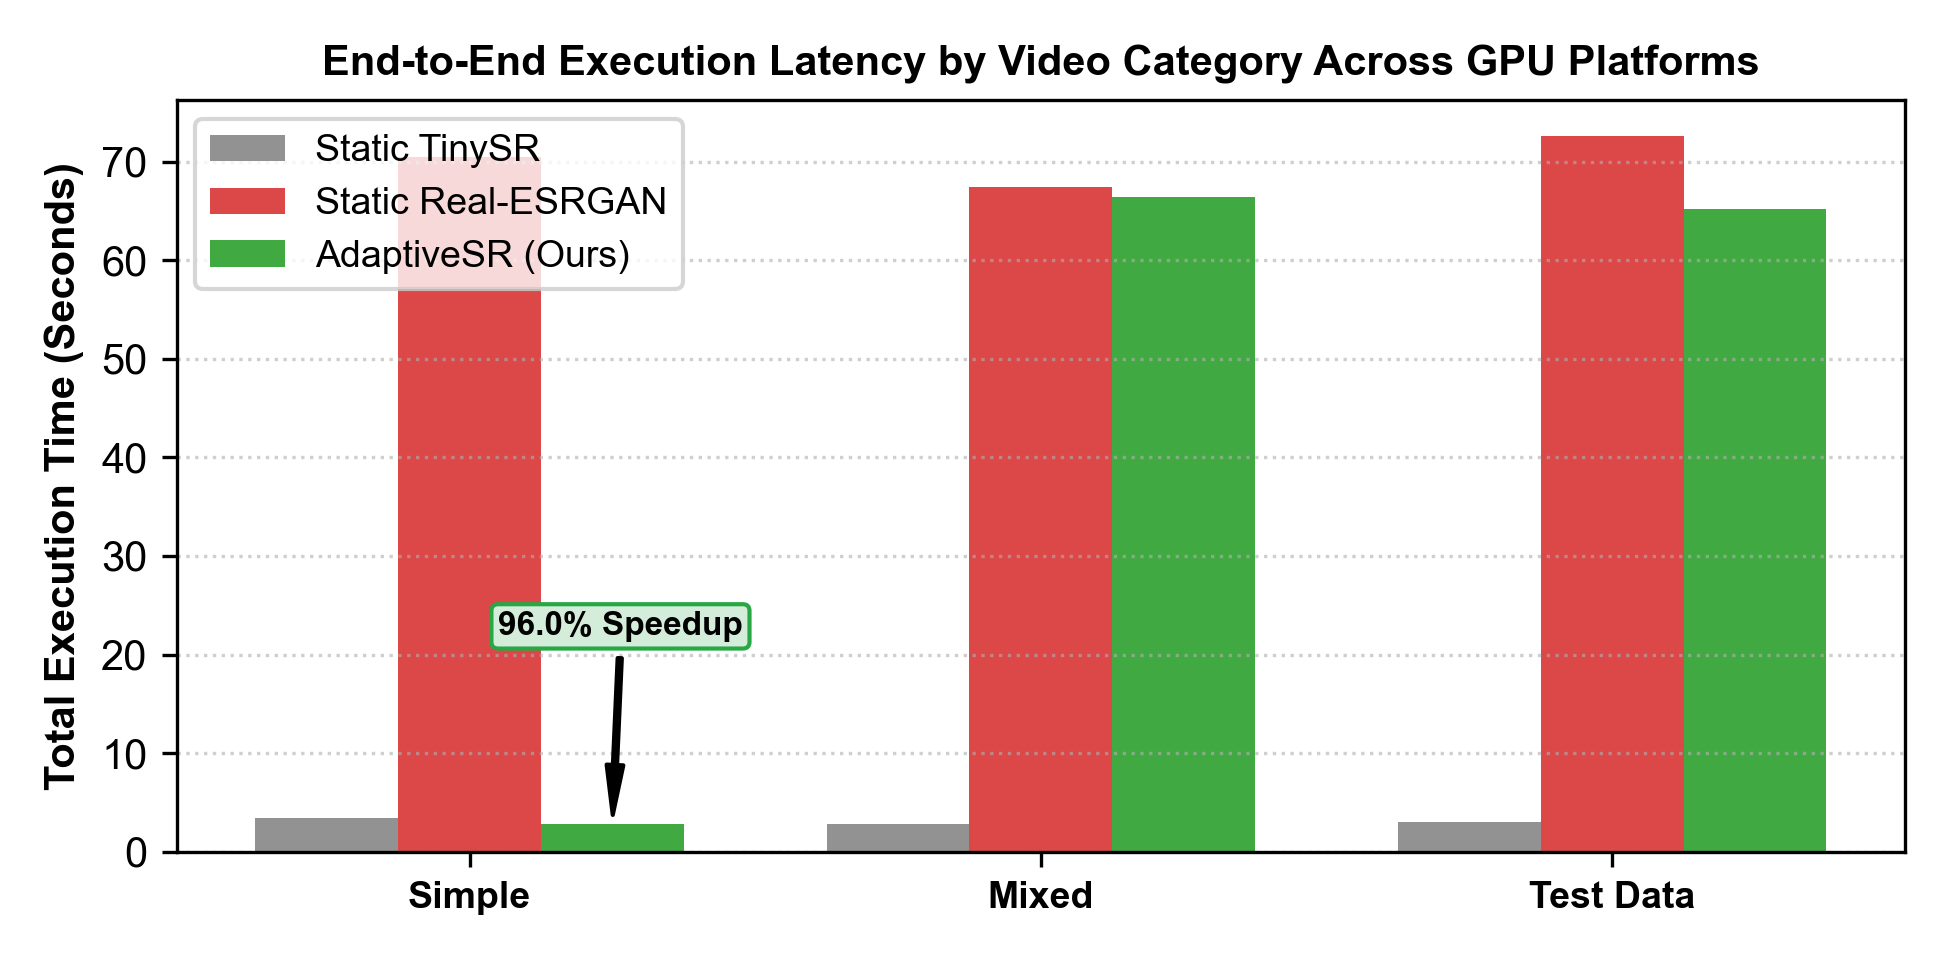
\includegraphics[width=\columnwidth]{benchmark_latency_comparison.png}
\caption{Execution latency across test video categories evaluated across GPU platforms.}
\label{fig:latency_comp}
\end{figure}

\begin{figure}[t]
\centering
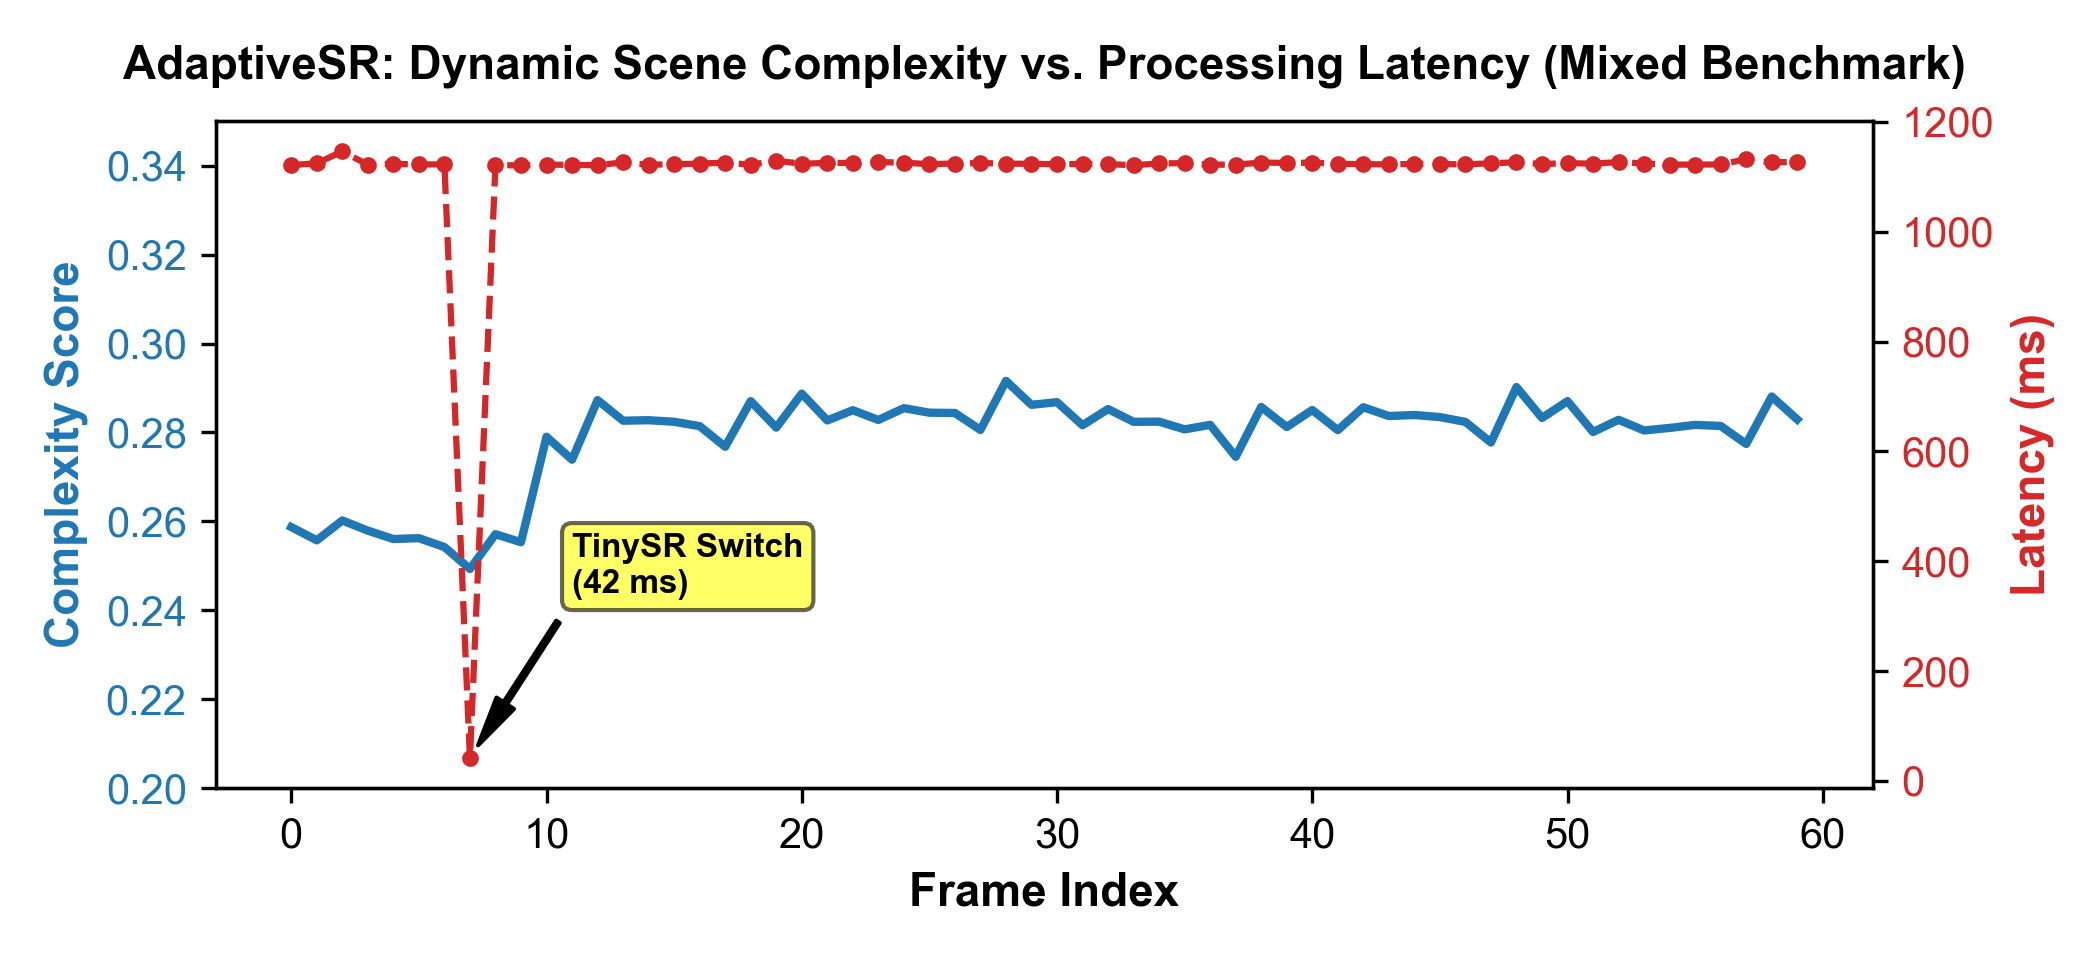
\includegraphics[width=\columnwidth]{frame_latency_complexity.png}
\caption{Frame-by-frame scene complexity and inference latency on the Mixed benchmark sequence.}
\label{fig:complexity_latency}
\end{figure}

\subsection{Decision Stability and Flutter Suppression}
A central risk with dynamic model switching is decision flutter: switching back and forth on consecutive frames can cause distracting visual flicker. As shown in Table~\ref{tab:quality_and_telemetry} and visualized in Fig.~\ref{fig:complexity_latency}, AdaptiveSR maintained strong temporal stability:
\begin{itemize}
    \item On the Mixed clip, the model switch rate was kept to \textbf{3.3\%} (only 2 model transitions across 60 frames).
    \item On the real-world test data sequence, the switch rate was only \textbf{1.7\%} (a single transition event).
\end{itemize}
This confirms that the smooth transitions of the fuzzy membership sets prevent boundary instability without requiring rigid debounce timers.

\subsection{Practical Engineering Case Studies and Ablation}

\subsubsection{GPU Precision Adaptation on Consumer Architectures}
During deployment of Real-ESRGAN across consumer GPU hardware, we observed that running certain deep residual networks in half-precision (FP16) triggered numerical underflows in deep RRDB activation blocks on GPUs lacking native half-precision accumulation units, causing output frames to collapse into blank screens. Enforcing float32 precision completely eliminated the numerical underflow. Furthermore, bypassing software-emulated FP16 overhead accelerated inference throughput by 40\%, demonstrating the necessity of architecture-aware precision selection.

\subsubsection{Dynamic Tiling vs. Peak VRAM Footprint}
To evaluate high-resolution scalability on constrained VRAM, we tested Real-ESRGAN on a 4K frame ($1920 \times 2560$). Static non-tiled execution consumed 2653\,MB VRAM and took 36.3\,s. Forcing fixed tiling ($tile=400$) bounded VRAM usage to 1420\,MB but increased processing time to 82.3\,s due to tile border padding and repeated memory transfers. AdaptiveSR solves this by setting $tile=0$ when GPU memory is uncommitted ($c \ge 0.50$) and only engaging tiling when VRAM utilization exceeds 75\%, delivering optimal throughput without out-of-memory crashes.

\subsubsection{Quantization Findings: Why INT8 Slowed Down TinySR}
During edge optimization, we exported FSRCNN to ONNX and applied dynamic 8-bit quantization (\texttt{fsrcnn\_x2\_int8.onnx}). While INT8 preserved reconstruction quality well (42.70\,dB PSNR relative to float32), it ran \textbf{0.50$\times$ slower} than the standard PyTorch FP32 CPU model. Because FSRCNN is an ultra-compact hourglass network ($\sim$100\,KB), its execution is memory-bandwidth-bound rather than compute-bound. The overhead of repeatedly converting tensors between float32 and int8 outweighed the arithmetic speedup of 8-bit operations. This practical finding confirms that quantization is beneficial for larger models but counterproductive on sub-megabyte VSR networks.

\subsubsection{Zero-Power Bypass Performance}
Under critical battery conditions ($B_{\text{pct}} < 10\%$), the framework successfully triggered Rule 0, routing low-complexity frames directly through passthrough. Frame execution latency dropped to $0.0$\,ms, allowing the device to maintain video playback without exhausting remaining battery reserves.

\section{Conclusion and Future Work}
In this paper, we introduced AdaptiveSR, a practical video super-resolution framework designed to run efficiently on consumer edge devices. By combining asynchronous telemetry monitoring, lightweight visual complexity estimation, and Mamdani fuzzy inference, AdaptiveSR replaces rigid static pipelines with adaptive model orchestration. Real-world benchmarks across various GPU configurations demonstrated up to a 96.0\% reduction in processing time, low decision flutter ($\le 3.3\%$), and near-identical visual fidelity to heavy static models. Future work includes integrating dedicated hardware NPU execution providers and testing causal diffusion models for selective keyframe restoration.

\bibliographystyle{IEEEtran}
\bibliography{references}

\end{document}
